\documentclass{standalone}
\usepackage{PhysicalChemistryNote}
\begin{document}
\begin{tikzpicture}
    \begin{axis}[
        width = 9cm,
        height = 6cm,
        legend pos = north east,
        xlabel = {$\dfrac{1}{\con{S}}$},
        ylabel = {$\dfrac{1}{v}$},
        axis lines = center,
        ymax = 4,
        ymin = 0,
        domain = -6:10,
        samples = 400,
        xticklabels={},
        yticklabels={}
    ]
    \addplot [thick, red, domain=1:10] {0.5*x+1};
    \addlegendentry{\small{No inhibitor}}
    \addplot [thick, cyan, domain=1:10] {0.25*x+1};
    \addlegendentry{\small{Competitive}}
    \addplot [thick, blue, domain=1:10] {0.5*x+2};
    \addlegendentry{\small{Uncompetitive}}
    \addplot [thick, violet, domain=1:10] {x+2};
    \addlegendentry{\small{Non-competitive}}
    \addplot [thick, red, dashed, domain=-2:1] {0.5*x+1};
    \addplot [thick, cyan, dashed, domain=-4:1] {0.25*x+1};
    \addplot [thick, blue, dashed, domain=-4:1] {0.5*x+2};
    \addplot [thick, violet, dashed, domain=-2:1] {x+2};
    \end{axis}
\end{tikzpicture}
\end{document}